\newcommand{\chapterpepperusecase}{Kapitel 6. }

\chapter{Implementierung: Anwendungsfälle}
\label{sec:Pepper_Anwendungsfaelle}
\lhead{\chapterpepperusecase \emph{Implementierung der Anwendungsfälle}}

%Im Folgenden werden wir auf die Implementierung unserer Anwendungsfälle eingehen. Hierbei gehen wir zuerst auf die Planung und anschließend auf die Bereitstellung der Daten in unserem Server und in externe Scripts ein. Anschließend erläutern wir die Implementation und Weiterverarbeitung der einzelnen Anwendungsfälle in Android Studio.\\
Im Folgenden werden wir auf die Implementierung und Weiterverarbeitung unserer Anwendungsfälle in Android Studio eingehen.\\


\section{Anzeigen der Mensadaten in Android Studio}

Pepper soll in der Lage sein, mit Hilfe von Sprache, den Mensaplan auf sein Tablet anzuzeigen und Informationen über die verschiedenen Angebote jedes Wochentags zu geben. Um sich den Mensaplan anzeigen zu lassen, haben wir zuerst ein neues Gesprächsthema in unserem Haupt-Topic erstellt. \\

\begin{lstlisting}[caption={Topic - Mensaplan}]
u:(["Ich hab{e} hunger" "Zeig {mir} {den} Mensaplan"] ) 
^execute(VariableExecutor, qiVariableMensa, Plan) Hier hast du eine 
Uebersicht ueber den Mensaplan
\end{lstlisting}

Sobald der Anwender nach dem Mensaplan fragt, wird die \verb|runWith| Methode mit den Parametern \verb|qiVariableMensa|
und \verb|Plan| in der \verb|VariableExecutor| Klasse aufgerufen.\\

\begin{lstlisting}[language=Python, caption={Übergabe der Parameter in runWith}]
case('qiVariableMensa'):
String day = params.get(1);
if(day.equals('Plan')){
    ...
}
\end{lstlisting}

In dieser Methode wird anschließend nach dem switch 
case \verb|qiVariableMensa| gesucht. Da wir einen zweiten Mensaanwendungsfall besitzen, müssen wir diese beiden Fälle  voneinander unterscheiden können. Aus diesem Grund wurde ein weiterer String Parameter mit dem Namen \verb|Plan| mitgegeben,  um über einer If-Bedingung diese beiden Fälle zu trennen. Nun gibt es mehrere Möglichkeiten, das Bild auf dem Tablet von Pepper anzeigen zu lassen. Die einfachste Methode wäre über den Webviewer. Hierfür hätten wir lediglich die URL benötigt, um die Webseite mit dem Bild auf dem  Tablet anzeigen zu lassen. Die Bildgröße des Mensaplans besaß jedoch eine viel zu große Auflösung (3200 x 4134 px), sodass nur ein Teil des Bildes auf dem Tablet angezeigt werden konnte. Auf dem Node Server oder in Android Studio könnte die Auflösung theoretisch manuell umgestellt werden, was wir jedoch vermeiden wollen. 

Wir haben uns anschließend für eine andere Lösung entschieden, wo das Bild in Android Studio als Bitmap vom Node Server heruntergeladen wird. Eine Bitmap ist eine Zahlenmatrix von einem Bild, wo jeder Pixel die jeweiligen Farbinformationen enthält.\\


\begin{lstlisting}[language=Java, caption={Bitmap im ContentView anzeigen}]
String url_str = "https://informatik.hs-bremerhaven.de/
docker-hbv-kms-http/api/v1/mensadata/img";
InputStream srt = new URL(url_str).openStream();
final Bitmap bitmap = BitmapFactory.decodeStream(srt);
    
ma.runOnUiThread(() -> {
    ma.setContentView(R.layout.mensa_layout);
    ImageView imageView = (ImageView) ma.findViewById(R.id.iMensa);
    imageView.setImageBitmap(bitmap);
});
\end{lstlisting}

In diesem Code wird das Bild in einen InputStream initialisiert. Ein InputStream ist eine Folge von Bytes, womit sich Daten lesen 
lassen können. Der InputStream wird mithilfe der \verb|BitmapFactory.decodeStream| Funktion in eine Bitmap umgewandelt. 
Anschließend kann eine Imageview mittels der Id mit der Bitmap initialisiert werden. 

Nun kann Pepper auf die Frage ``Zeig mir den Mensaplan'' ein Bild von dem aktuellen Mensaplan auf sein Tablet zeigen. \\

\begin{figure}[H]
    \centering
    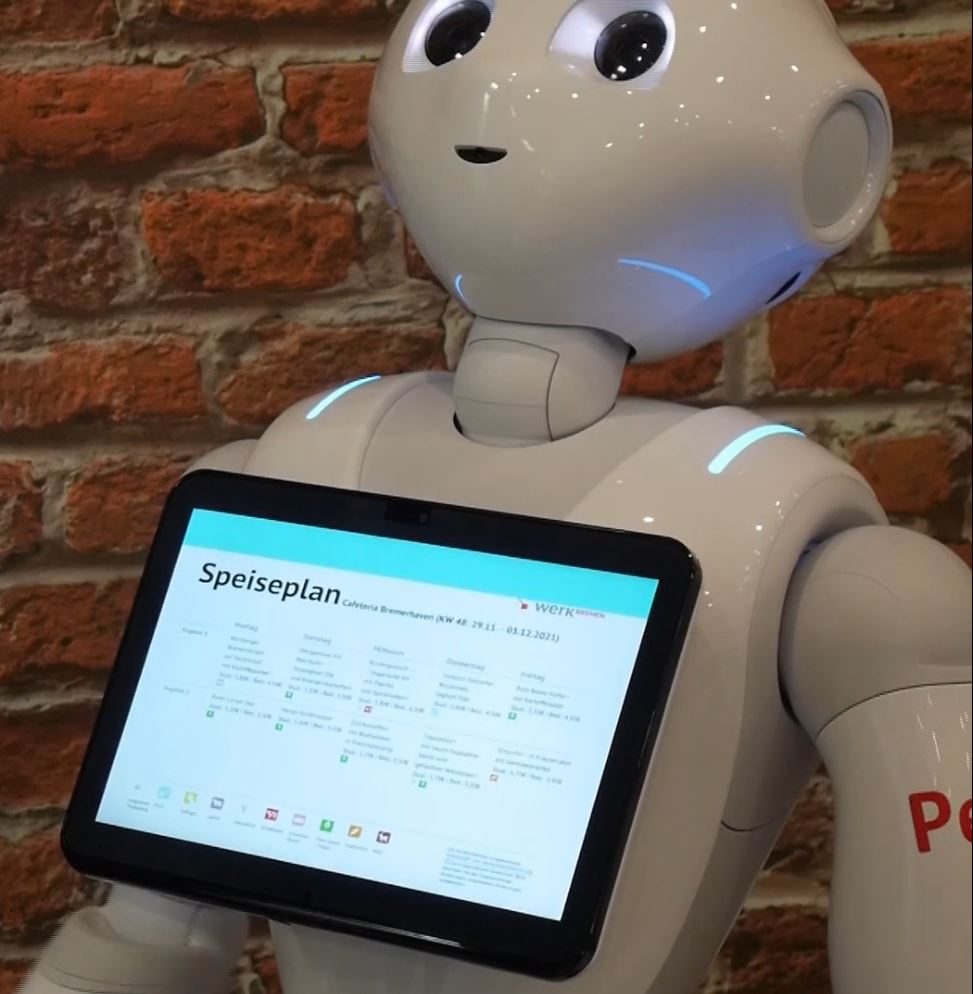
\includegraphics[width=6cm]{Figures/AppChapter/rx2.JPG}
    \caption{Mensaplan auf Hopper}
    \label{fig:mensaplanPepper}
    \centering
\end{figure}

Als Nächstes wird ein weiteres Gesprächsthema erstellt, dass Pepper erlaubt, auch verbal Informationen über die Mensa Angebote zu geben.\\

\begin{lstlisting}[caption={Topic - Mensadaten}]
concept:(week) [Montag Dienstag Mittwoch Donnerstag 
Freitag Heute Morgen Uebermorgen]

u:({was} {gibt{s}} {es} {zu} essen {am} _[~week]) $day=$1 
^execute(VariableExecutor, qiVariableMensa, $day) $day gibt 
es entweder $qiVariableMensa

u:({was} {gibt{s}} {es} {am} _[~week] {zu} essen) $day=$1 
^execute(VariableExecutor, qiVariableMensa, $day) $day gibt 
es entweder $qiVariableMensa
\end{lstlisting}

Hier wird die Variable \verb|day| mit dem Wochentag in  \verb|_[~week]| initialisiert, dass in der Frage genannt wurde. Wenn der Anwender zum Beispiel fragt: ``Was gibt es am Mittwoch zu essen'', wird Mittwoch in die Variable \verb|day| initialisiert. In dem Konzept wurden nicht nur Wochentage, sonder auch Wöter wie Heute, Morgen und Übermorgen hinzugefügt. Somit kann der Anwender auch fragen, was es zum Beispiel morgen zu essen gibt. Anschließend wird wieder die \verb|runWith| Methode aufgerufen mit den Parameter \verb|qiVariableMensa| und dem Wochentag, der genannt wurde. In der VariableExecutor Klasse wird nun die Antwort vorbereitet, die Pepper zu der Frage geben soll. Hierfür wird die \verb|getOffer| Methode in 
der HelperCollection Klasse aufgerufen.\\

\begin{lstlisting}[language=Java, caption={Auslesen der Mensa-API}]
HttpURLConnection con = getConnection("https://informatik.
hs-bremerhaven.de/docker-hbv-kms-http/api/v1mensadata");

BufferedReader in = new BufferedReader(new InputStreamReader(
    con.getInputStream()));
String inputLine;
StringBuffer response = new StringBuffer();
while ((inputLine = in.readLine()) != null) response.append(inputLine); 
in.close();

JSONObject myResponse = new JSONObject(response.toString());
String tmp = myResponse.getString("offer1");
String [] offer1 = tmp.split("\",\"", -1);
tmp = myResponse.getString("offer2");
String [] offer2 = tmp.split("\",\"", -1); 
\end{lstlisting}

Zuerst werden die Daten aus dem Server aufgerufen und mithilfe des \verb|BufferedReader| in das \verb|StringBuffer| Objekt \verb|response| initialisiert. Anschließend wird ein JSON Objekt aus dem \verb|response| erstellt. Für uns war es leichter, die Daten in einem Array zu speichern, weshalb wir zwei Arrays mit den jeweiligen Mensa Angeboten initialisiert haben.\\

\begin{lstlisting}[language=Java, caption={Kalenderfunktion in Java}]
Calendar calendar = Calendar.getInstance();
int curday = calendar.get(Calendar.DAY_OF_WEEK) - 2;    
\end{lstlisting}

Nun wird mit der Calendar Bibliothek von Java, der aktuelle Wochentag ermittelt und als Zahl in curday gespeichert. Wäre der aktuelle Wochentag ein Montag, so würde curday mit einer 0 initialisiert. Sollte es ein Mittwoch sein, dann wäre curday eine 2 usw. Somit können wir die Arrays \verb|offer1| und \verb|offer2| mit dem genauen Index des aktuellen Wochentags ermitteln.\\

\begin{lstlisting}[language=Java, caption={Ermittlung der Mensadaten für heute, morgen und übermorgen}]
String [] daylist = {
    "Montag", "Dienstag", "Mittwoch", "Donnerstag", "Freitag"
};

String [] spcdays = {"Heute", "Morgen", "Uebermorgen"};
String answer = "";

for(int i = 0; i < spcdays.length; ++i){
    if(day.equals(spcdays[i])){
        if((curday + i) > 5){
            answer ="Am Wochenende ist die Mensa leider geschlossen";
            break;
        }
        
        answer = offer1[curday + i].replaceAll("\"", "").replace(
            "[","").replace("]",""
        );

        answer += " oder " + offer2[curday + i].replaceAll("\"", "")
            .replace("[","").replace("]",""
        );
        break;
    }
}    
\end{lstlisting}

In der For-Schleife wird das Array \verb|spcdays| iteriert und mit \verb|if(day.equals(spcdays[i]))| wird anschließend überprüft, ob der Anwender das Angebot für Heute, Morgen oder Übermorgen wissen möchte. Außerdem wird 
überprüft, ob der Anwender mit der Frage Morgen oder Übermorgen den Freitag überschreitet. Sollte der Wochentag zum Beispiel ein Freitag 
sein und der Anwender würde fragen, was es morgen in der Mensa zu essen gibt, dann wird Pepper antworten, dass die Mensa am Wochenende geschlossen 
ist. Sollte der Tag in der Woche sein, so wird die Antwort in der Variable \verb|answer| mit den beiden Angeboten initialisiert. \\

\begin{lstlisting}[language=Java, caption={Ermittlung der Mensadaten für bestimmte Wochentage}]
for(int i = 0; i < daylist.length; ++i){
    if(day.equals(daylist[i])){
        answer = offer1[i].replaceAll("\"", "").replace("[","")
            .replace("]","");
        answer += " oder " + offer2[i].replaceAll("\"", "")
            .replace("[","").replace("]","");
        break;
    }
}
\end{lstlisting}

Diese For-Schleife überprüft, ob der Anwender das Mensaangebot für einen bestimmten Wochentag wissen will. Dementsprechend wird dann die 
Antwort initialisiert.\\

\begin{lstlisting}[language=Python]
String offer = HelperCollection.getOffer(day);
ma.getCurrentChatBot().setQiVariable(variableName, offer);    
\end{lstlisting}

Nachdem nun alle Antworten vorbereitet wurden, wird die Variable “qiVariableMensa” mit der Antwort initialisiert und in den Topic 
zurückgegeben. \\

\begin{figure}[H]
    \centering
    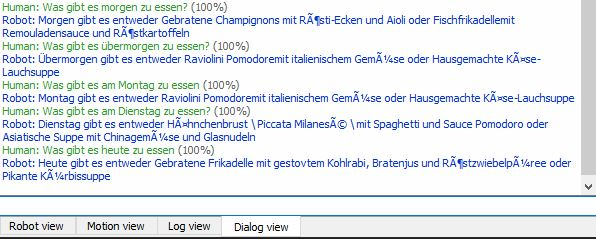
\includegraphics[width=\textwidth]{Figures/AppChapter/mensa_6.JPG}
    \caption{Mensa Dialog}
    \label{fig:mensadialog}
    \centering
\end{figure}


\section{Anzeigen des Stundenplans in Android Studio}
Der zweite Anwendungsfall ist das Anzeigen des Stundenplans für jeden Studiengang und für jedes Semester. \\
Die Bereitstellung der Stundenplandaten im Node Server wurde bereits im Abschnitt \ref{sec:api-timetable} erläutert. Nun war es und möglich, auf diese Daten in Android Studio, über ein GET Request, zuzugreifen und weiterzuverarbeiten. Das Ziel ist es, den Stundenplan über die WebView anzeigen zu lassen. 
\\
Hierfür wurde ein neues Gesprächsthema in dem Haupt-Topic erstellt.\\

\begin{lstlisting}[caption={Topic - Stundenplan}]
u:({so} zeig{e} {er} {mir} {den} Stundenplan {fuer} {den} Studiengang 
_~Studiengaenge {[im "fuer das"]} semester _~semester {sofort} {bitte})

$course=$1 $semester=$2 Alles klar ^execute(VariableExecutor, 
timetable_course_semester, $course, $semester)
\end{lstlisting}

Damit der Anwender den Stundenplan einsehen kann, erwartet Pepper zwei Wörter. Der Anwender muss in seiner Frage den Studiengang und das Semester 
nennen. Erst dann wird der Methodenaufruf gestartet. Somit werden die drei Parameter \verb|timetable_course_semester|, 
\verb|course| und \verb|semester| mitgegeben.\\

\begin{lstlisting}[language=Java, caption={Studiengang und Semester ermittlung}]
final String timetableurl = "https://informatik.hs-bremerhaven.de/
    docker-hbv-kms-http/api/v1/timetable?course="
    + course_ + "&semester="
    + semester_ + "&htmlOnly=true";

ma.runOnUiThread(() -> {
	ma.setContentView(R.layout.webtest);

	WebView web = (WebView) ma.findViewById(R.id.webView);
	WebSettings webSettings = web.getSettings();
	webSettings.setJavaScriptEnabled(true);
	web.setWebViewClient(new Callback());
	web.loadUrl(url);
});
\end{lstlisting}

Auf dem Node Server erwartet die API, die wir für den Stundenplan erstellt haben, bestimmte Parameter zu dem Studiengang und dem Semester. Hierfür können wir unsere Parameter, die in der Frage ermittelt wurden, in die Variable \verb|timetableurl| einsetzen und erhalten die URL zu dem richtigen Stundenplan. Dieser kann anschließend mit Hilfe des Webviewers auf dem Tablet von Pepper angezeigt werden. \\


\section{Anzeigen des Gebäudeplans und des Raumfinders in Android Studio}

Der dritte und letzte Anwendungsfall ist die Navigationshilfe in der Hochschule Bremerhaven. Sollte der Anwender einen bestimmten Raum oder ein Gebäude suchen, soll Pepper auf seinem Tablet eine genaue Wegbeschreibung geben können. 
\\
Da wir die einzelnen Videodateien auf dem Hopper abgelegt haben, brauchen wir für diesen Anwendungsfall die Kommunikation mit dem Node Server nicht. 

Um auf die einzelnen Informationen der Raumdaten zugreifen zu können, wurde eine externe JSON Datei erzeugt, der diese beinhaltet. Die Erstellung dieser Datei wird im Abschnitt \ref{sec:jsonget} näher erläutert. Die Datei wurde im /Assets Ordner in Android Studio abgelegt, um sie später im Code verwenden zu können. 

Wie bei allen anderen Anwendungsfällen auch, ist der erste Schritt das Erstellen der einzelnen Gesprächsthemen. 
Zuerst werden wir den Fall abdecken, wenn sich der Anwender den Gebäudeplan anzeigen lassen will.\\

\begin{lstlisting}[caption={Topic - Raumfinder}]
u:([zeig gib] {mir} {bitte} {den} [Gebaeudeplan Campusplan Gelaende])
^execute(VariableExecutor, qiVariableNav, Plan) Hier hast du eine 
    Uebersicht ueber das Hochschulgelaende
\end{lstlisting}


\begin{lstlisting}[language=Java, caption={Anzeigen des Gebäudeplans}]
String nav = params.get(1);
if(nav.equals("Plan")) {
    try {
        ma.runOnUiThread(() -> { ma.setContentView(R.layout.campus_plan); });
    } catch (Exception e) { e.printStackTrace(); }
}
\end{lstlisting}

(vgl. Abb. \ref{fig:gplan}) Sobald der Anwender nach dem Gebäudeplan fragt, wird ein vordefiniertes XML-Layout mit einem Bild von dem 
Gebäudeplan auf dem Tablet angezeigt. Das Bild wurde vorher heruntergeladen und in den Ordner 
\verb|drawable| gelegt.\\

\begin{figure}[H]
    \centering
    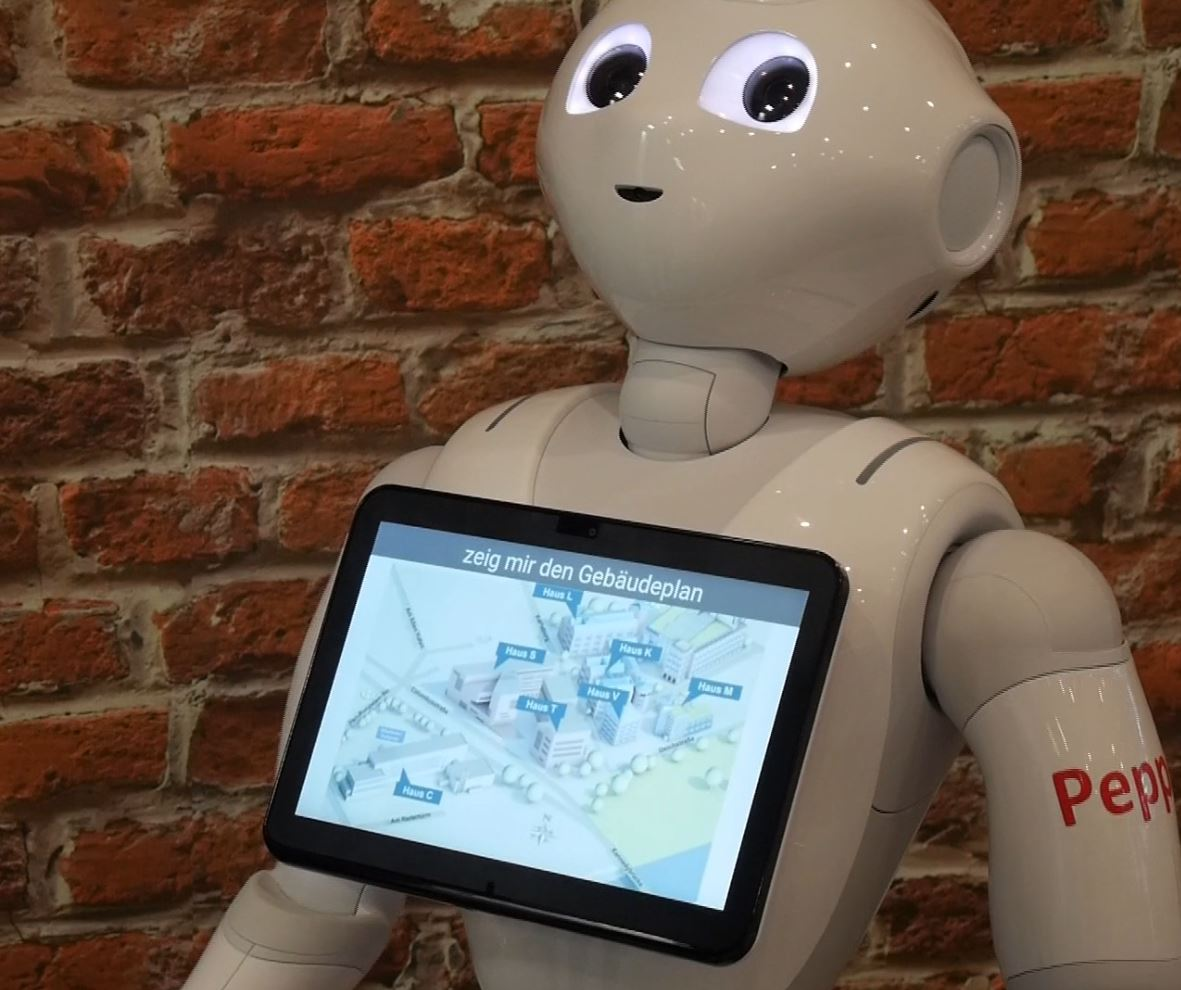
\includegraphics[width=10cm]{Figures/AppChapter/rx3.JPG}
    \caption{Gebäudeplan - Pepper}
    \label{fig:gplan}
    \centering
\end{figure}

Als Nächstes haben wir das Abrufen der Videodateien zu den einzelnen Räumen der Hochschule in Android Studio implementiert.\\

\begin{lstlisting}[caption={Konzept für jeden Raum inder Hochschule Bremerhaven}]
concept:(rooms) [C006 C007 ... Z5150 Z5160 ]

u:(["{Kannst du {mir} [sagen erzaehlen]} Wo [befindet ist] {sich} der 
Raum _~rooms {befindet}"])
    $room=$1 Sofort ^execute(VariableExecutor, qiVariableNav, $room)
\end{lstlisting}

Pepper muss in der Lage sein, alle Räume in der Hochschule zu kennen, um genau herausfiltern zu können, welchen Raum der Anwender sucht. Das Concept \verb|rooms| beinhaltet alle Räume der Hochschule und wird somit in der Frage im Topic verwendet. Sollte der Anwender nach einen Raum fragen, den es nicht gibt, wird Pepper die Frage erst gar nicht verstehen und nicht antworten. 

Sollte Pepper den Raum kennen, wird ein Methodenaufruf mit den Parametern \verb|qiVariableNav| und der Raumnummer (\verb|room|) durchgeführt.\\
\newpage
\begin{lstlisting}[caption={Topic - Barrierefrei}]
u:(Zeig mir {bitte} einen _~handicapped Weg [zu in] {dem} 
Raum _~rooms)
    $handicap=$1 $room=$2 Alles klar ^execute(VariableExecutor, 
    qiVariableNav, $room, $handicap)
\end{lstlisting}

Wenn der Anwender explizit nach einem barrierefreien Weg zu einem Raum fragt, wird der gleiche Methodenaufruf mit dem zusätzlichen Parameter \verb|handicap| durchgeführt.\\

\begin{lstlisting}[language=Java, caption={Optioanle Barrierefreiheit}]
String room = nav;
String handicapped = "M0000";
if(params.size() == 3) handicapped = "M0001";
\end{lstlisting}


In der \verb|VariableExecutor| Klasse wird als Erstes überprüft, ob der Anwender nach einem barrierefreien Weg zu dem gewünschten Raum gefragt hat oder nicht. Mit der If-Bedingung wird die Länge der Parameter überprüft, die in der Methode mitgegeben wurde. Wie bereits erwähnt, wird ein zusätzlicher Parameter \verb|handicap| zusammen mit den Parametern \verb|qiVariableNav| und \verb|room| mitgegeben, wenn nach dem barrierefreien Weg gefragt wurde. Somit muss nur die Parameterlänge verglichen werden, um entscheiden zu können, welcher Weg angezeigt werden soll.\\

\begin{lstlisting}[language=Java, caption={Auslesen der Routenfinder Daten}]
BufferedReader reader = new BufferedReader(new InputStreamReader(
    ma.getAssets().open("route_metadata.json")));
String response = new String();
for (String line; (line=reader.readLine())!=null; response+=line);
Map jsonJavaRootObject = new Gson().fromJson(response, Map.class);
String path = ((Map)((Map)(jsonJavaRootObject.get(room)))
    .get(handicapped)).get("video_path").toString();
\end{lstlisting}

Mit der \verb|getAssets().open("route_metadata.json")| Funktion, kann die JSON Datei, die sich in dem \verb|/assets| Ordner befindet, geöffnet und mit dem \verb|BufferedReader| ausgelesen werden. Als Nächstes wird mit Hilfe des \verb|Gson| Frameworks, ein Map Objekt erzeugt, dass alle Informationen der JSON Datei bereitstellt. In der Variable \verb|path|, wird der Wert 
\verb|video_path| mit Hilfe der genauen Raumnummer herausgefiltert. Hier wird auch die Abfrage mitgegeben, ob der Weg Barrierefrei sein soll oder nicht.\\

\begin{lstlisting}[language=Java, caption={Darstellung der Wegbeschreibung auf Peppers Tablet}]
String urlVideo = "https://informatik.hs-bremerhaven.de/hbv-kms/" + path;
try{
    ma.runOnUiThread(() -> {
        ma.setContentView(R.layout.webtest);
        WebView web = (WebView) ma.findViewById(R.id.webView);
        WebSettings webSettings = web.getSettings();
        webSettings.setJavaScriptEnabled(true);
        web.setWebViewClient(new Callback());
        web.loadUrl(urlVideo);
    });
}
\end{lstlisting}

(vgl. Abb. \ref{fig:Routenfinder}) Nachdem der genau Pfad zum Video ermittelt wurde, kann nun die URL zu dem Video erstellt und mit dem Webviewer angezeigt werden.\\

\begin{figure}[H]
    \centering
    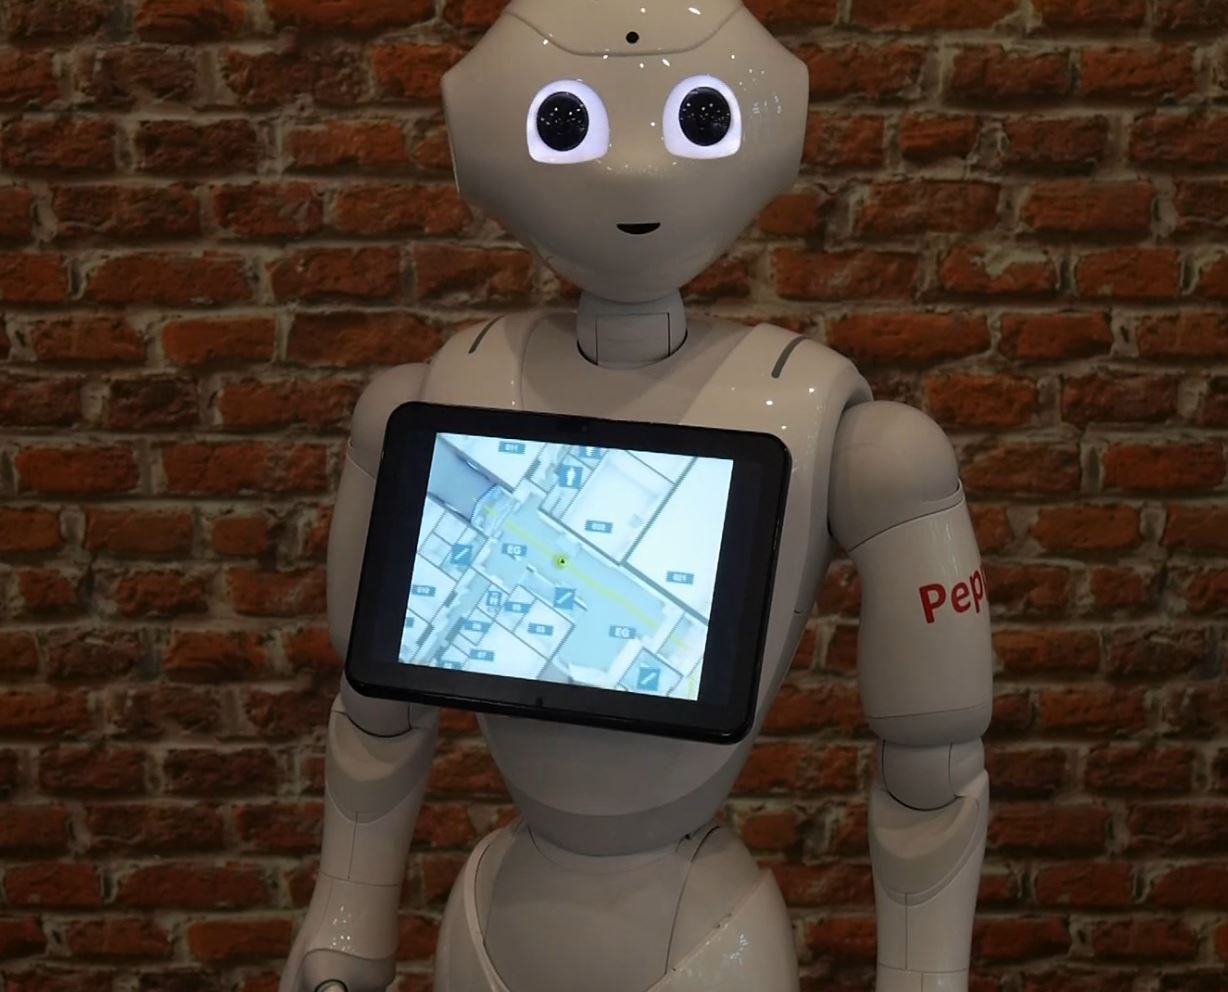
\includegraphics[width=10cm]{Figures/AppChapter/rx4.JPG}
    \caption{Routenfinder}
    \label{fig:Routenfinder}
    \centering
\end{figure}

(vgl. Abb. \ref{fig:RoutenfinderDia}) Zusätzlich zu dem Video soll Pepper dem Anwender mit zusätzlichen Details antworten. Er gibt an, in welchem Gebäude sich der gesuchte Raum befindet, 
wie weit dieser von seinem Standpunkt entfernt ist und wie viel Zeit benötigt wird, um diesen Raum zu erreichen.\\

\begin{figure}[H]
    \centering
    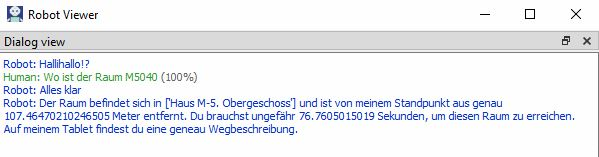
\includegraphics[width=\textwidth]{Figures/AppChapter/raumfinder_1.JPG}
    \caption{Routenfinder Dialog}
    \label{fig:RoutenfinderDia}
    \centering
\end{figure}

